
\title{Rover}

\date{\today}

\author{Alex Wallar}

\documentclass[12pt]{article}

\usepackage{amsmath}

\usepackage[pdftex]{graphicx}

\usepackage{relsize}

\usepackage{float}

\usepackage{algorithm}

\usepackage[noend]{algorithmic}

\floatstyle{ruled} \newfloat{program}{thp}{lop} \floatname{program}{Structure}

\newcommand{\Normal}[3]{\mathcal{N}(#1, #2, #3)}

\newcommand{\Acronym}[1]{\ensuremath{{\small{\texttt{#1}}}}}
\newcommand{\Constant}[1]{\ensuremath{\small{\texttt{#1}}}}
\newcommand{\Rover}{\Acronym{Rover}}
\newcommand{\Keeper}{\Acronym{Keeper}}
\newcommand{\False}{\Constant{false}}
\newcommand{\True}{\Constant{true}}
\newcommand{\Symbol}[1]{\ensuremath{\mathcal{#1}}}
\newcommand{\Function}[1]{\ensuremath{{\small \textsc{#1}}}}
\newcommand{\Var}[1]{\ensuremath{{\small{\textsl{#1}}}}}
\newcommand{\argmin}[1]{\underset{#1}{\operatorname{arg}\,\operatorname{min}}\;}
\newcommand{\grad}[1]{\underset{#1}{\operatorname{\Function{GradientDecent}}}\;}

\newcommand{\fig}[1]{\textbf{Figure \ref{fig:#1}}}

\usepackage{fancyvrb}

\begin{document}

\maketitle

\newpage

% \tableofcontents

% \newpage

\section{Introduction}

Unmanned aerial vehicles, such as quadcopters, are becoming a cheap and
feasible way to provide persistent monitoring of an area even when monitoring
that area comes with a risk of the quadcopter being detected by possibly
hostile parties. These quadcopters are left unattended and need to be able to
plan their movements autonomously such that they maximize the quality of their
sensors and maintain as much sensor coverage as possible, whilst minimizing the
risk of being apprehended. The autonomous planning also needs to take into
account that some quadcopters will be dispatched from the swarm to follow
certain targets of interest. The planning algorithm should be able to
organically readjust the swarm such that maximum sensor quality and minimum
risk are preserved and should provide a method of tracking the targets of
interest by a sub-swarm.

The proposed solution, Rover, provides a method of organically readjusting the
swarm to fill the search space whilst maximizing sensor quality and sensor
coverage while minimizing the risk by combining dynamic potential fields and
convex optimization.

\section{Rover}

Rover is an planning algorithm that seeks to maximize the sensor quality and
sensor coverage for a group of quadcopters, whilst minimizing the risk of a
quadcopter being detected by a possibly hostile enemy. This is done by
splitting the planning into two different parts, planning for the 2D plane to
promote sensor coverage and planning for the altitude by minimizing risk and
maximizing sensor quality.

\subsection{2D Planning}

For the 2-dimensional planning, Rover needs to make sure that the group of
quadcopters fills the search space and guarantee that no one part of the space
goes too long without being surveyed. This is done by discretizing the space
into a grid. Whenever a box in the grid has been covered by a sensor on any
quadcopter in the group, the current time is stored in that box.  For the
quadcopters to move in the $xy$ plane, each quad will sample a given number
points along its sensor radius. It will then move in the direction of the box
in the grid that has the lowest time (in seconds) recorded. This simple rule
has extreme emergent properties for the swarm. Since the swarm shares the same
grid, the quads will act cooperatively to fill the space without having to
provide much guidance. This is shown in \fig{cover}. Also, this planning is not
dependent on how many quads there are in the swarm. If a quad leaves the swarm,
it would simply no longer update the time grid. The other quads would have no
knowledge that it left and would still be able to plan accordingly. Also this
style of planning inherently follows the rules of a swarm; distance is
maintained between boids, boids tend towards their neighbours headings, and
boids that are two far away will get closer together.


\begin{figure}

\begin{center}

$$ \begin{array}{cc}

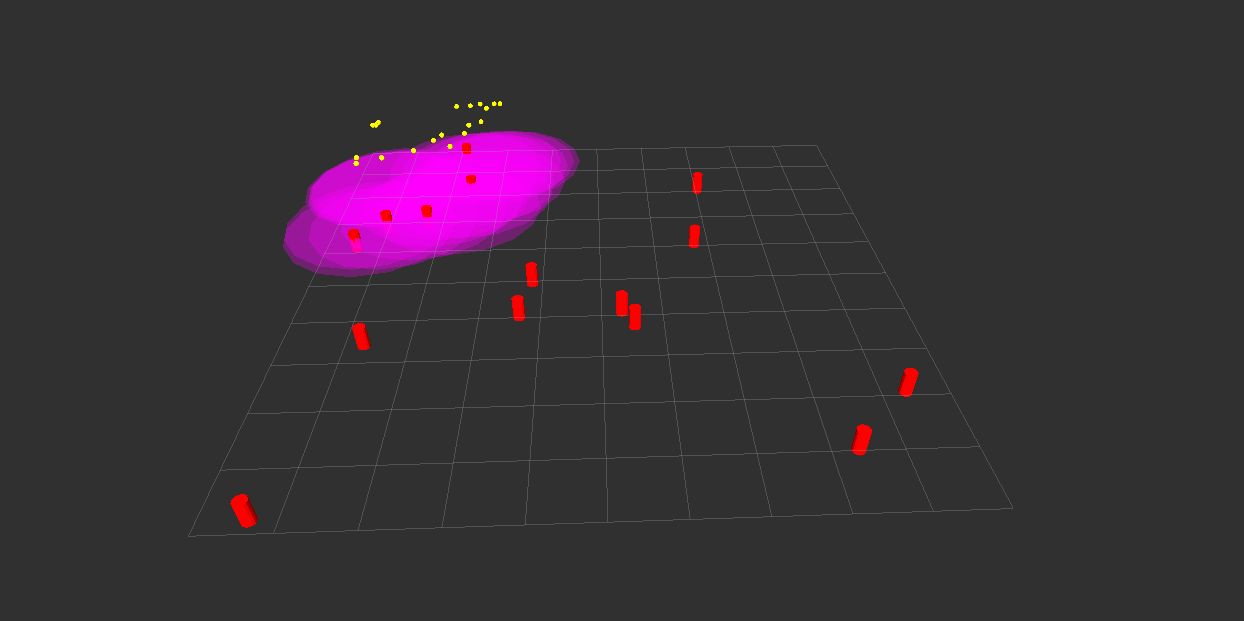
\includegraphics[width=2.5in]{figs/rover1.png} &

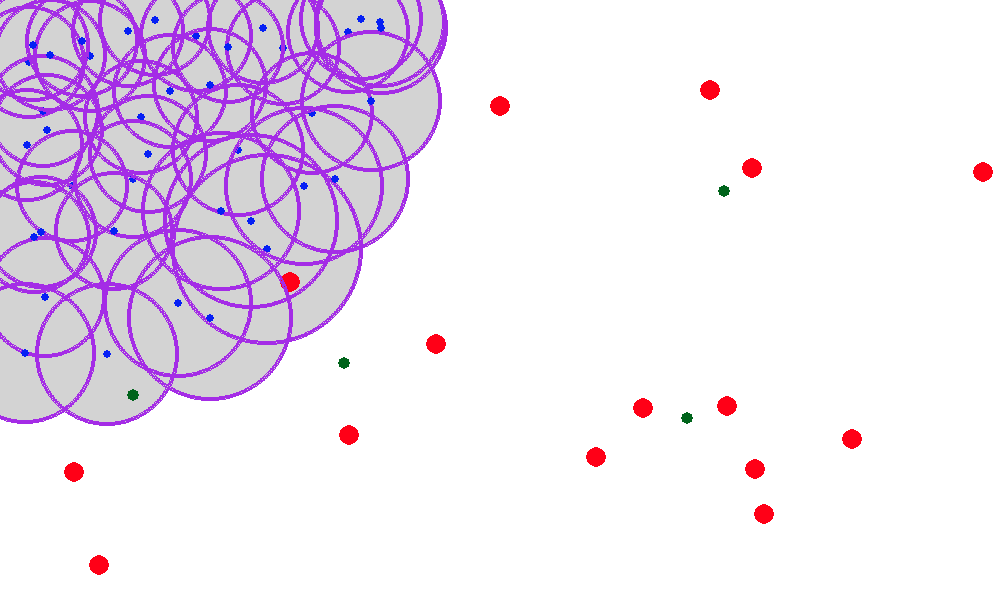
\includegraphics[width=2.5in]{figs/rover2.png} \\

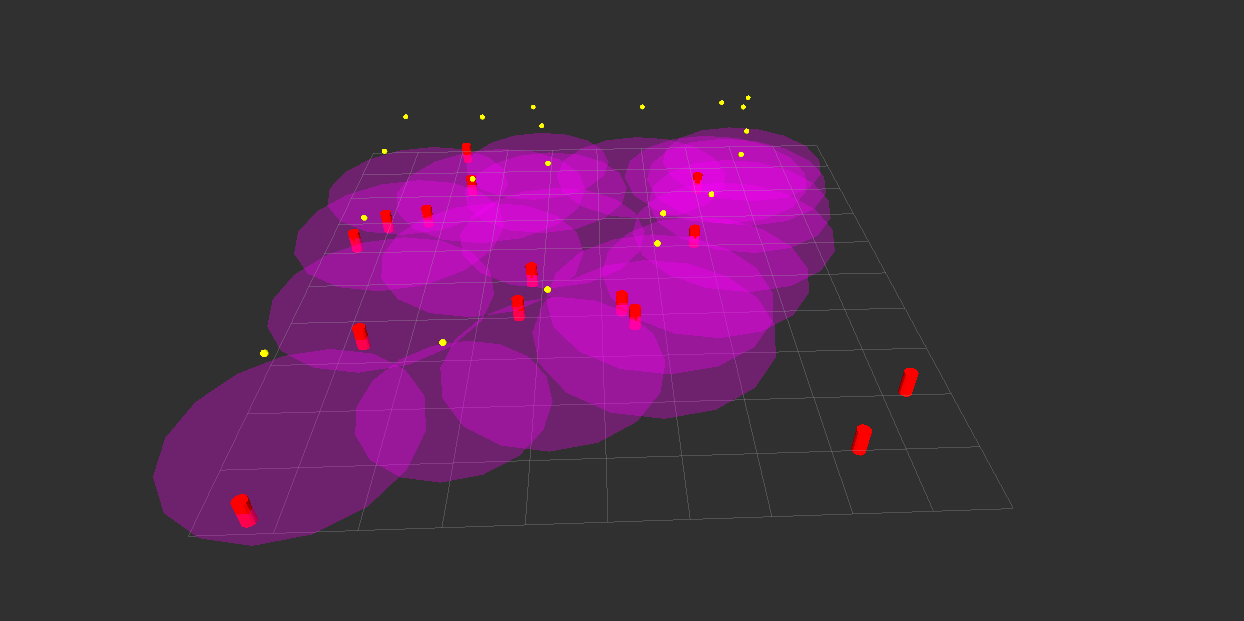
\includegraphics[width=2.5in]{figs/rover3.png} &

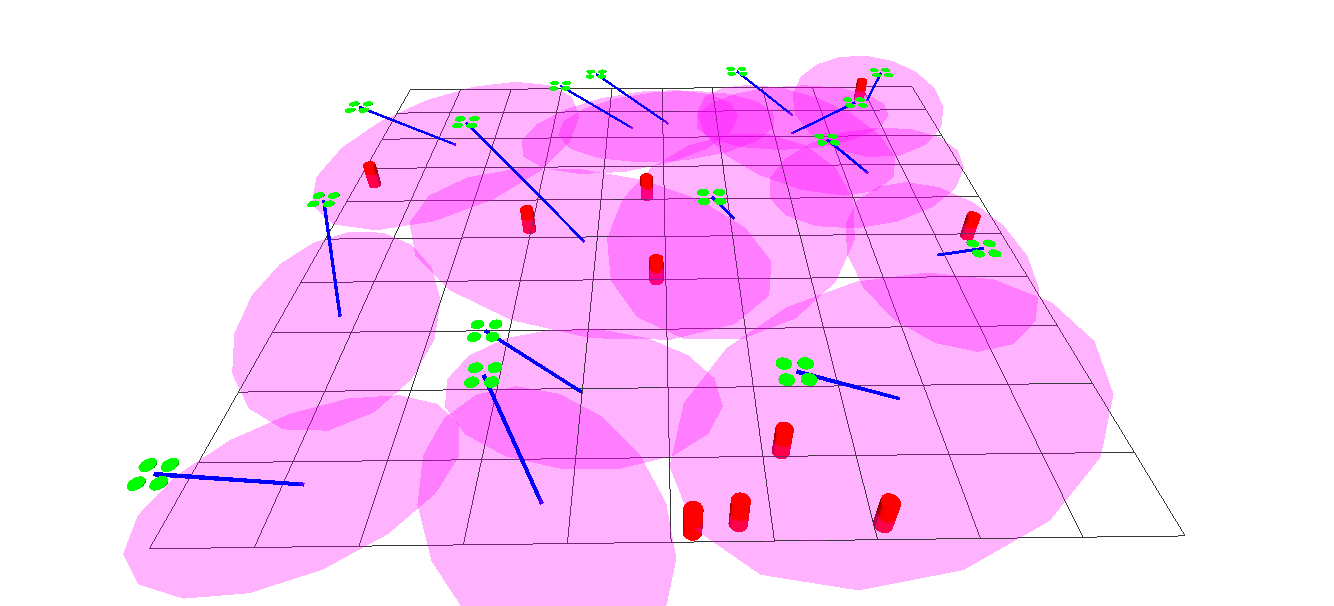
\includegraphics[width=2.5in]{figs/rover4.png}

\end{array} $$

\end{center}

\caption{2D Coverage}

\label{fig:cover}

\end{figure}

\subsection{Determining the altitude}

To determine the altitude, one must solve a convex optimization problem that
tries to optimize the height of the quad by maximizing the sensor quality and
minimizing the risk. This is done by modeling the sensor quality and the risk
as concave functions. This solution works given the assumption that as the quad
increases altitude, the sensor quality will degrade however the sensor radius
will increase. The "thought" sensor so to speak used in development was a
camera.

\paragraph{Sensor Quality} The function for sensor quality is fairly straight
forward.  Imagine a down facing camera on a quadcopter with a strict viewing
angle. The sensor quality will be a relative measurement comparing how much
data is represented by the image captured at the minimum height and how much
data is represented at some given height. This is done by mapping the size of
the viewing circle at the minimum height to the given height. After reducing
the equations, sensor quality is modeled by an elegant inverse square function
shown below.

$$ SQ(z) = \frac{z_{min} ^ 2}{z ^ 2} $$

\paragraph{Risk} The function for risk is more complicated and is based on
empirical observation. This function (like that of sensor quality) can be
substituted for another one that meets the user's need. Risk is measured based
on two things, the initial risk at an $x, y$ position, and the height of the
quad. The initial risk is the risk at the minimum altitude. This is measured by
dispersing points of high risk within the space (the red dots in \fig{cover})
and using a Gaussian distribution to model the risk. Using this initial risk, a
secondary function is created that models how the risk decreases as the height
increases. Please note that the convex optimization does not occur with risk,
but however the percentage of initial risk. This is to make the sensor quality
function and risk model have a nice intersection point. To determine the actual
risk at a given spot, one simply multiplies the initial risk to the percentage
of initial risk function. Given an initial risk, the risk model describes the
risk as the percentage of initial risk. By changing the initial risk at a
point, one changes this function, which leads to a different solution from the
convex optimization. The function for risk is shown below.

$$ R(z) = 1 - (\frac{z - z_{min}}{r_0 \cdot (z_{max} - z_{min})}) ^ 2 $$

\paragraph{Optimization}

By solving for $z$ in $SQ(z) - R(z) = 0$, we are able to determine the height
needed for the quadcopter such that sensor quality is maximized and risk is
minimized. This can be solved with many open source solvers. The package being
used in this implementation is SciPy. Once the altitude needed for the quad has
been determined, the new height is set and the time grid is updated. This means
that given the new height, and therefore a new sensor radius, neighbouring
quads will move away if the height has increases so to not overlap sensing
areas, and if the height has decreased, the neighbouring quads will move
towards the given quad.

\subsection{Future Work}

Rover needs to be ported to ROS and to be tested with real quadcopters in a
practical, real world setting. Once Rover has been ported to ROS, more
algorithms can be developed using the data that has been collected by the
quadcopters. Using the data collected by the quads, realtime 2D collaborative
mapping could be achieved. This would give vital information to groups of
robots on the ground about their surroundings. Also, creating a suite of
classifiers that can be used to determine the position of a critical target and
use Keeper to interpolate its movement throughout the space. Moreover using
these classifiers, Rover could build risk maps in realtime and relay them back
to the groups of robots on the ground.  This could provide vital information
that could limit the risk exposure of troops on the ground.

\end{document}
